\section{Test01: GPU vs CPU}
The results of this test are used as baseline for further optimizations. \\
Test configuration:
\begin{itemize}
  \item \textbf{CPU}: Intel(R) Core(TM) i7-4770K CPU @ 3.50GHz 
  \item \textbf{GPU}: NVIDIA Tesla K40c 
\end{itemize}
Implementations tested:
\begin{itemize}
  \item \textbf{legacy\_multifit\_cpu}: plain \textit{cms-sw} cpu code.
  \item \textbf{legacy\_multifit\_gpu}: plain gpu porting \textit{cms-sw} cpu code.
  \item \textbf{multifit\_cpu}: inplace fnnls cpu implementation.
  \item \textbf{multifit\_gpu}: inplace fnnls gpu implementation.
  \item \textbf{multifit\_cpu\_swap}: fnnls cpu implementation with swapping matrices.
  \item \textbf{multifit\_gpu\_swap}: fnnls gpu implementation with swapping matrices.
\end{itemize}
\begin{figure}[h]
  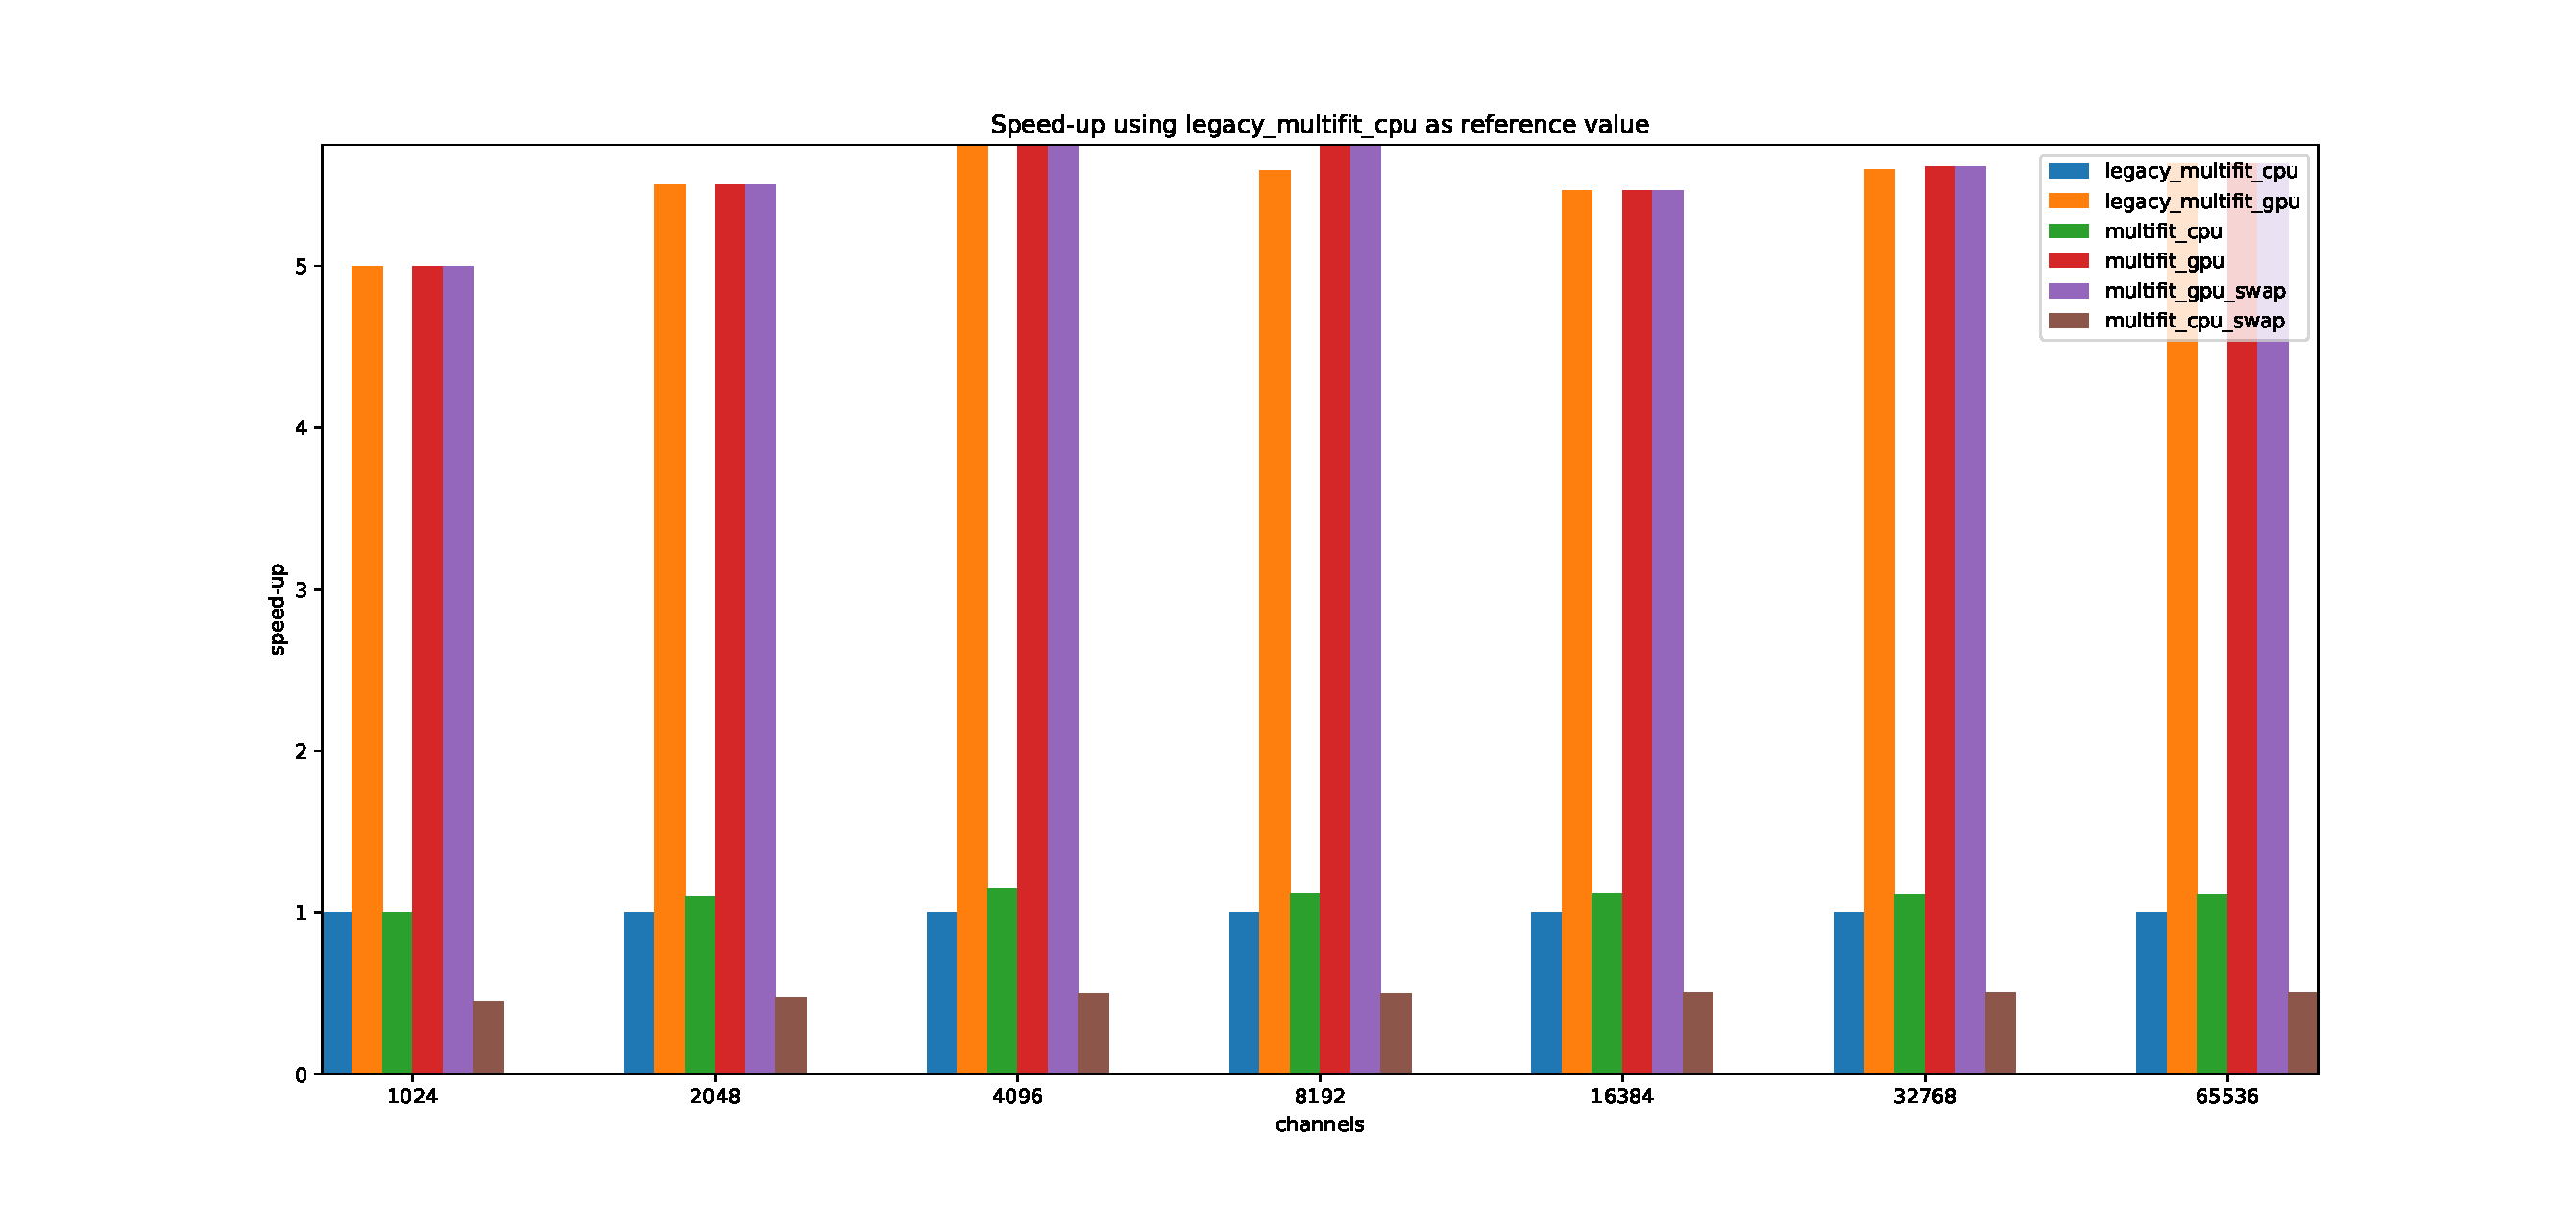
\includegraphics[width=\textwidth]{img/speedup}
  \caption{Speedup achieved with 10 iterations, higher is better}
  \label{img:speedup01}
\end{figure}
All the cpu implementations are single-threaded. With 64k channels the optimized GPU version achieves a speedup of $2.67$. Since the corresponding CPU version achieves a speedup of $1.10$, the GPU implementation runs more than twice as fast as the corresponding CPU one.
\begin{figure}[H]
  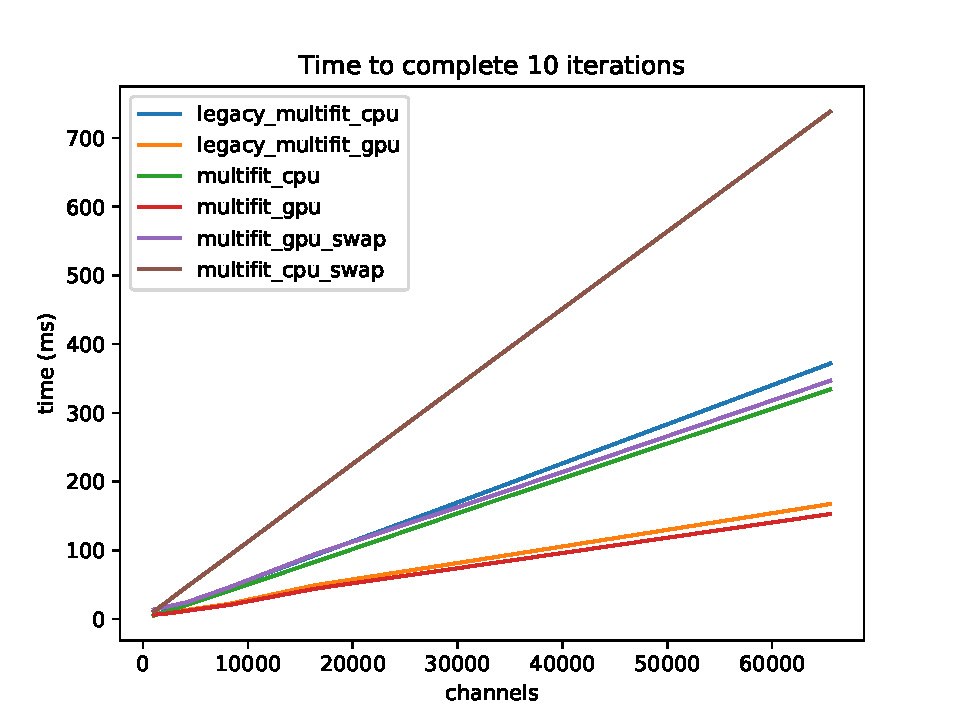
\includegraphics[width=.75\textwidth]{img/linscale}
  \caption{Time needed to complete 10 iterations, linear channel scale, lower is better}
  \label{img:linscale01}
\end{figure}
From \ref{img:speedup01} that the GPU performs almost six times as fast with respect to the CPU. Other optimizations like loop unrolling and branch reduction give a performance gain about 20\% on CPU.
\begin{figure}[H]
  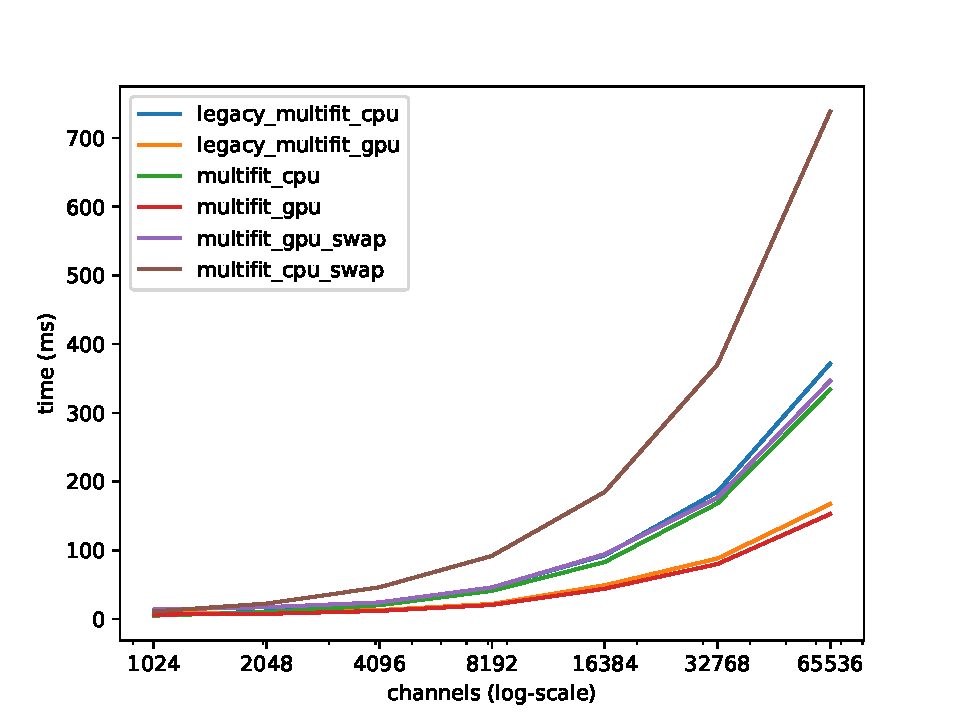
\includegraphics[width=.75\textwidth]{img/logscale}
  \caption{Time needed to complete 10 iterations, log channel scale, lower is better}
  \label{img:logscale01}
\end{figure}
From the plot present in \ref{img:linscale01} can be noted that in the GPU version there is a change of slope around 15k channels, after this number the growth slows-down.
The plot in \ref{img:logscale01} makes more evident the difference between the different version of the algorithm. The GPU outperforms the CPU and since the growth is sub-linear, it will be interesting to study what will happen if the number of channels increases even more.\\
\section{Test02: GPU vs CPU, Optimized Matrix multiplication}

\begin{figure}[h]
  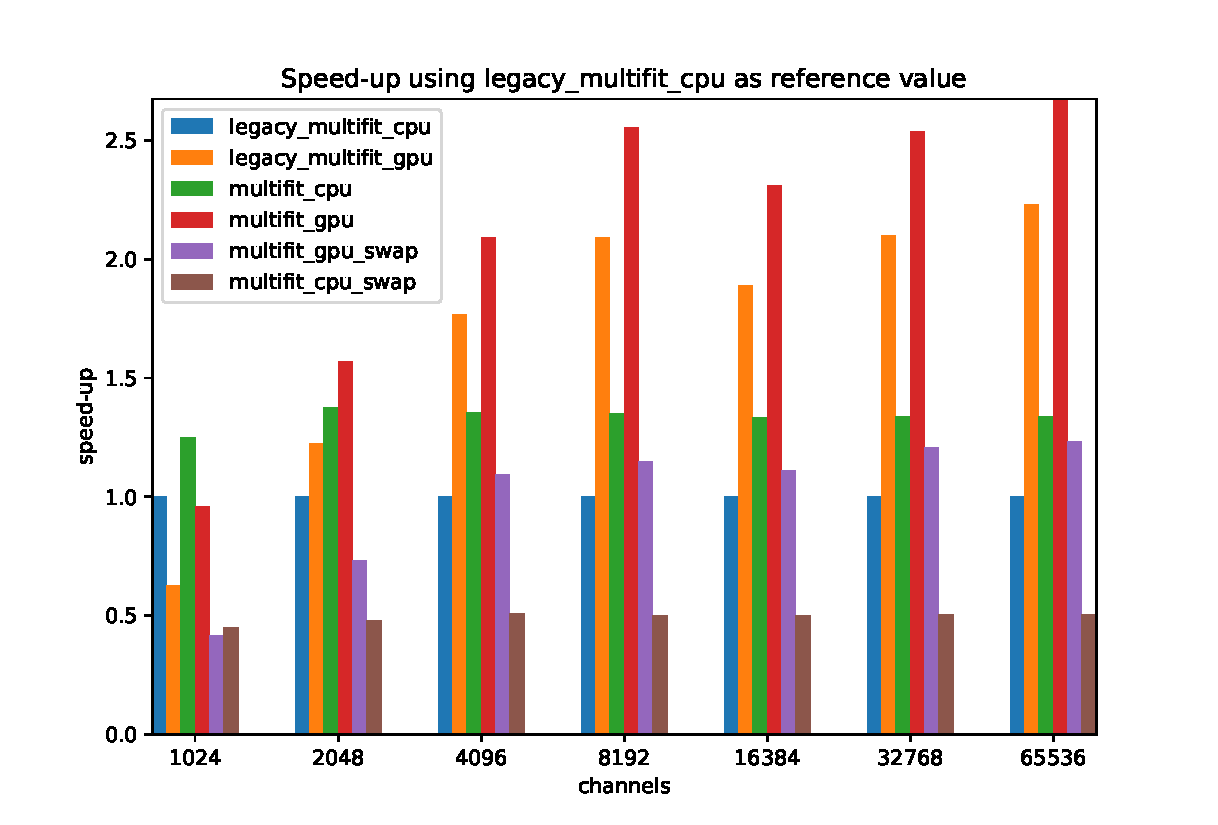
\includegraphics[width=\textwidth]{img/speedup02}
  \caption{Speedup achieved with 10 iterations, higher is better}
  \label{img:speedup02}
\end{figure}
All the cpu implementations are single-threaded. With 64k channels the GPU version achieves a speedup of 5.8 that it the same as the previous test.
\begin{figure}[H]
  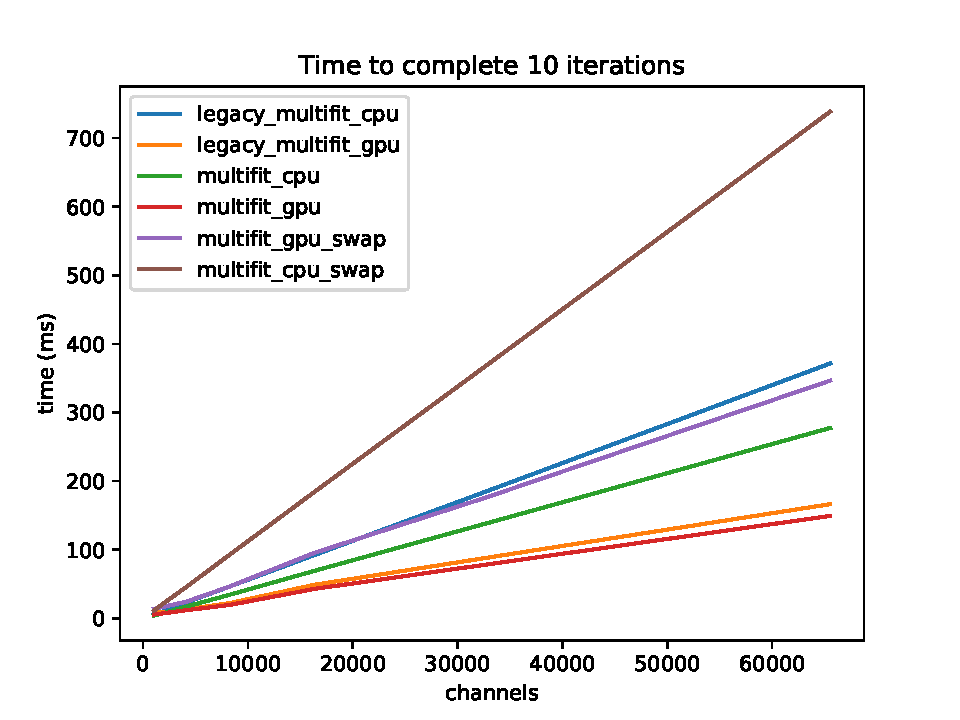
\includegraphics[width=.75\textwidth]{img/linscale02}
  \caption{Time needed to complete 10 iterations, linear channel scale, lower is better}
  \label{img:linscale02}
\end{figure}
From \ref{img:speedup01} can be noted that even with all the optimizations the GPU speedup it does not increase. This is due to the fact that the GPU is underutilized so even if the implementation requires less resources it can not be noted in this test, and the data transfer respect to the computation is very big. The optimized CPU implementation in this case performs $35\%$ better than the legacy one.
\begin{figure}[H]
  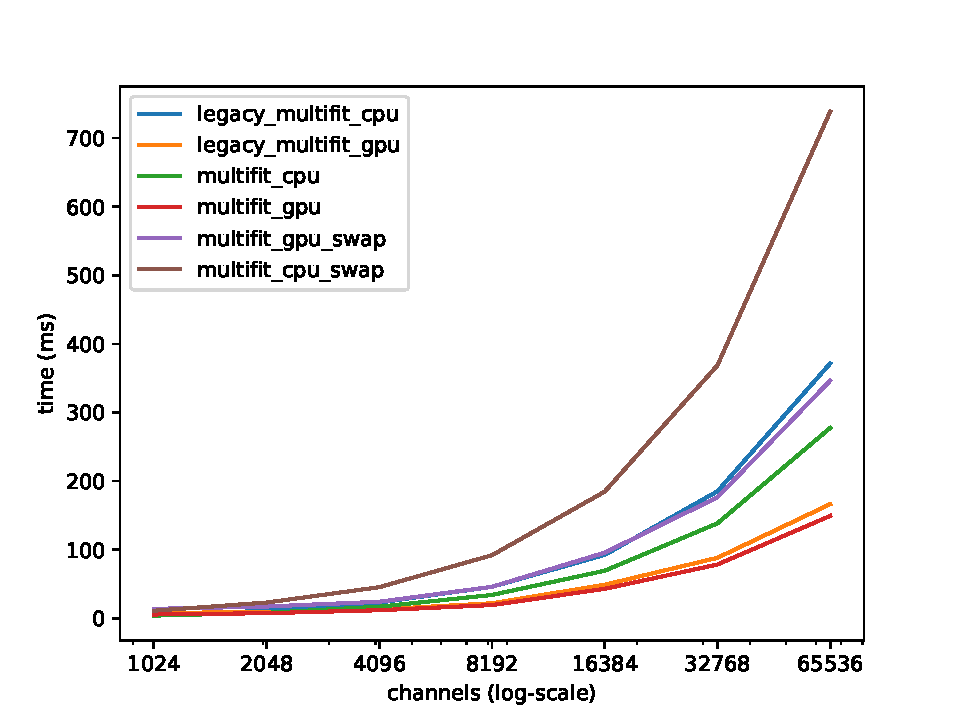
\includegraphics[width=.75\textwidth]{img/logscale02}
  \caption{Time needed to complete 10 iterations, log channel scale, lower is better}
  \label{img:logscale02}
\end{figure}